\documentclass[tikz, border=5pt]{standalone}

% Required packages
\usepackage{pgfplots}
\usepackage{pgfplotstable}
\usepackage{tikzviolinplots}
\pgfplotsset{compat=1.18}

\usepackage{cite}
\usepackage{amsmath,amssymb,amsfonts}
\usepackage{algorithmic}
\usepackage{graphicx}
\usepackage{textcomp}
\usepackage{xcolor}
\usepackage{tikz}
\usepackage{physics}
\usepackage{algorithm}
\usepackage{pgfplots}
\usepackage{pgfplotstable}
% \usepackage[sorting=none]{biblatex}
\usepgfplotslibrary{statistics}
\usepackage{etoolbox} % for \ifnumcomp
\usepackage{listofitems} % for \readlist to create arrays
% \usepackage[ruled,vlined]{algorithm% Increase row height
\renewcommand{\arraystretch}{1.4}

% Adjust column spacing
\setlength{\tabcolsep}{8pt}  % default is 6pt, increasing it for better spacing

\tikzset{>=latex} % for LaTeX arrow head
\colorlet{myred}{red!80!black}
\colorlet{myblue}{blue!80!black}
\colorlet{mygreen}{green!60!black}
\colorlet{mydarkred}{myred!40!black}
\colorlet{mydarkblue}{myblue!40!black}
\colorlet{mydarkgreen}{mygreen!40!black}
\tikzstyle{node}=[very thick,circle,draw=myblue,minimum size=22,inner sep=0.5,outer sep=0.6]
\tikzstyle{connect}=[->,thick,mydarkblue,shorten >=1]
\tikzset{ % node styles, numbered for easy mapping with \nstyle
  node 1/.style={node,mydarkgreen,draw=mygreen,fill=mygreen!25},
  node 2/.style={node,mydarkblue,draw=myblue,fill=myblue!20},
  node 3/.style={node,mydarkred,draw=myred,fill=myred!20},
}
\def\nstyle{int(\lay<\Nnodlen?min(2,\lay):3)} % map layer number onto 1, 2, or 3

\usetikzlibrary{arrows.meta,shadows,positioning}
\usetikzlibrary{calc}
\usetikzlibrary{fit, positioning, shapes.geometric}
\tikzset{
	frame/.style={
		rectangle, draw,
		text width=6em, text centered,
		minimum height=4em,drop shadow,fill=white,
		rounded corners,
	},
	line/.style={
		draw, -{Latex},rounded corners=3mm,
	}
}
% Tikz Library
\usetikzlibrary{calc, quotes, angles}
\pgfmathsetmacro{\r}{0.8}
\pgfmathsetmacro{\Phi}{-160}
\pgfmathsetmacro{\Theta}{-90}
\usepackage{fontawesome5}
\usepackage{float}
% \def\BibTeX{{\rm B\kern-.05em{\sc i\kern-.025em b}\kern-.08em
%     T\kern-.1667em\lower.7ex\hbox{E}\kern-.125emX}}








    \begin{document}

% \begin{figure}[H]
% 	\centering
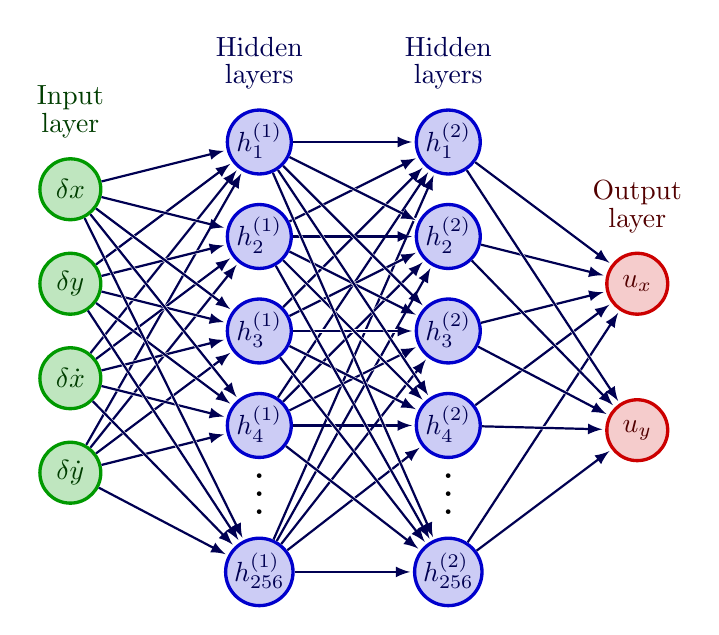
\begin{tikzpicture}[x=2.4cm,y=1.2cm]
	\readlist\Nnod{4,5,5,2} % array of number of nodes per layer
	\readlist\Nstr{n,256,k} % array of string number of nodes per layer
	\readlist\Cstr{x,h^{(\prev)},u} % array of coefficient symbol per layer
	\def\yshift{0.55} % shift last node for dots
	
	% LOOP over LAYERS
% LOOP over LAYERS
\foreachitem \N \in \Nnod{
  \def\lay{\Ncnt} % alias of index of current layer
  \pgfmathsetmacro\prev{int(\Ncnt-1)} % number of previous layer
  \foreach \i [evaluate={\c=int(\i==\N); 
  \layercheck=\ifnum\Ncnt=1 0 \else \ifnum\Ncnt=\Nnodlen 0 \else \yshift \fi \fi;
  \y=\N/2-\i-\c*\layercheck;
  \x=\lay; \n=\nstyle;
  \index=(\i<\N?int(\i):"\Nstr[\n]");}] in {1,...,\N}{ % loop over nodes
    % NODES
	\ifnum \lay=1
	\ifnum \i=1
		\node[node \n] (N\lay-\i) at (\x,\y) {$\delta x$};
	\fi
	\ifnum \i=2
		\node[node \n] (N\lay-\i) at (\x,\y) {$\delta y$};
	\fi
	\ifnum \i=3
		\node[node \n] (N\lay-\i) at (\x,\y) {$\delta {\dot{x}}$};
	\fi
	\ifnum \i=4
		\node[node \n] (N\lay-\i) at (\x,\y) {$\delta {\dot{y}}$};
	\fi
	\else \ifnum \lay=\Nnodlen
	\ifnum \i=1
		\node[node \n] (N\lay-\i) at (\x,\y) {$u_x$};
	\fi
	\ifnum \i=2
		\node[node \n] (N\lay-\i) at (\x,\y) {$u_y$};
	\fi
	\else
    \node[node \n] (N\lay-\i) at (\x,\y) {$\strut\Cstr[\n]_{\index}$};
    \fi \fi
    % CONNECTIONS
    \ifnumcomp{\lay}{>}{1}{ % connect to previous layer
      \foreach \j in {1,...,\Nnod[\prev]}{ % loop over nodes in previous layer
        \draw[white,line width=1.2,shorten >=1] (N\prev-\j) -- (N\lay-\i);
        \draw[connect] (N\prev-\j) -- (N\lay-\i);
      }
    %   \ifnum \lay=\Nnodlen
    %     \draw[connect] (N\lay-\i) --++ (0.5,0); % arrows out
    %   \fi
    }{
    %   \draw[connect] (0.5,\y) -- (N\lay-\i); % arrows in
    }
  }

  % Dots (skip first and last layers)
  \ifnum \lay>1 \ifnum \lay<\Nnodlen
    \path (N\lay-\N) --++ (0,1+\yshift) node[midway,scale=1.6] {$\vdots$}; % dots
  \fi \fi
}

  
	
	% LABELS
	\node[above=.1,align=center,mydarkgreen] at (N1-1.90) {Input\\[-0.2em]layer};
	\node[above=.1,align=center,mydarkblue] at (N2-1.90) {Hidden\\[-0.2em]layers};
	\node[above=.1,align=center,mydarkblue] at (N3-1.90) {Hidden\\[-0.2em]layers};
	\node[above=.1,align=center,mydarkred] at (N\Nnodlen-1.90) {Output\\[-0.2em]layer};
  \end{tikzpicture}
%   \caption{Neural network architecture of the actor in the DDPG algorithm.}
%   \label{fig:actor_nn}
% \end{figure}


\end{document}